\documentclass[a4paper,12pt,twocolumn]{article}
\usepackage[utf8]{inputenc}
\usepackage[english]{babel}

\usepackage{graphicx}
\usepackage{color}
\usepackage{transparent}
\usepackage
    % [showframe=true] % uncomment this line to show the lines
    {geometry}

\geometry{verbose,tmargin=20pt, bmargin=60pt
    , lmargin=30pt, rmargin=30pt
}

\begin{document}
% remove all indents from new paragraphs
% \setlength{\parindent}{0pt}

\title{
    Growing A Tetris Player with Big Data\\
    \large Project Report by Group 22
}
\author{
    \bf{Li Jiaxin Cassandra}\\ 
    A0131652N
    \and
    \bf{Loh Han Tong, Victor}\\
    A0135808B
    \and
    \bf{Ryan Tan Wen Jun}\\
    A0135747X
    \and
    \bf{Tan Yu Wei}\\
    A0142255M
}
\date{\today}
\maketitle

\section{Introduction}
The purpose of this project is to create a utility based agent to maximise the
number of rows removed in a game of Tetris. This tetris playing agent uses a heuristic
function to estimate the utility of each state.

% In this report, we discuss how this agent was designed and the features used to
% evaluate the utility of the board. We will also look at how we have implemented
% and used genetic algorithm to train a tetris agent that could play Tetris decently well,
% averaging about 19,700,000 lines cleared. 
In this report, we discuss the design and strategies used in the agent, and how our
agents learnt better strategies through Genetic Algorithm (Section \ref{features_subsection}, \ref{genetic}).
We will then look at how we have tackled speeding up gameplay (Section 2.3) and the
results of our learnt agent's performance in a standard game (Section 3). Lastly,
we discuss our findings and other possible extensions.

% TODO: Other things we can elaborate further: ==> Refer to the sections of report!
% In this report, we discuss the design and strategies used in the agent, and how we got
% agents with better strategies through Genetic Algorithms (Section 2.1, 2.2)
% we will then look at how we have tackled speeding up gameplays (Section 2.3)
% results of how well our learnt agent performs in a standard game (Section 3)
% etc etc

% Intuitively, for GA ==> Think of it as a battle arena of a 1000 individualparticipants

\section{Strategy}
The agent's heuristic function sums the linear weights $w(k)$ of features $\varphi_k(s)$
(As stated in Section \ref{features_subsection}) for a given state of the board,
\textit{s}, where \textit{n} is the number of features as shown below:

\[
    \hat V(s) = \sum_{k=0}^{n}w(k)\varphi_k(s)
\]

Where at every turn, the agent evaluates all possible moves and makes the move
that gives the best utility.

\subsection{Features Selected}
\label{features_subsection}
This is the list of 11 features that we have selected. They allow us to
evaluate each state \textit{s} based on certain characteristics of the board.

\begin{itemize}
    \item \textbf{NUM\_ROWS\_REMOVED} -- Number of rows removed after each action
    \item \textbf{MAX\_HEIGHT} -- Height of the tallest column
    \item \textbf{TOTAL\_HEIGHT} -- Sum of all column heights
    \item \textbf{TOTAL\_DIFF\_HEIGHT} -- Sum of all difference in height of all columns
    \item \textbf{LANDING\_HEIGHT} -- Height of where the lowest point of next piece lands
    \item \textbf{NUM\_HOLES} -- Number of empty cells with at least one filled cell above
    \item \textbf{COL\_TRANSITION} -- Number of filled cells adjacent to empty cells,
        summed over all columns
    \item \textbf{ROW\_TRANSITION} -- Same as the above, but applied to rows
    \item \textbf{COVERED\_GAPS} -- Number of empty cells with a filled cell
        anywhere above them
    \item \textbf{TOTAL\_WELL\_DEPTH} -- Sum of the depth of all wells
    \item \textbf{HAS\_LOST} -- Gives a penalty of -10000 if move result in loss,
        else give 100
\end{itemize}

Intuitively, the weight vector can be thought of as the agent's strategy on
the board, based on the features it sees. For example, if the agent has a weight
vector that gives a high positive weight value to TOTAL\_DIFF\_HEIGHT, it will have
a general strategy to always prefer moves that increases the overal "bumpiness" of
the tetris wall.

This gives us a clear way in interpreting the values from the weight vector and how
it corresponds to the overall strategy of the agent.

\subsection{Genetic Algorithm}
\label{genetic}
For our implementation of the genetic algorithm, Each chromosome has a weight
vector where each gene (weight value) corresponds to one of the 11 features
stated in Section \ref{features_subsection}, and a fitness score.


The fitness score of each chromosome is defined as the mean score of playing 50
games using that individual's chromosome weight.

This is a simple summary of our implementation of the genetic algorithm:
\begin{enumerate}
    \item Start out with 1000 individuals with random weights, let this be the population pool.
    Calculate the fitness score of all of the individuals in the population.
    \item Select 40\% of population via Stochastic Universal Sampling to be
            potential parents, let this be the parent pool.
    \item Generate 40\% of population as offsprings and put them into an offspring pool
    by the process below:
        \begin{enumerate}
            \item Randomly select 2 parents from the parent pool generated above
            \item Crossover with 80\% chance, by taking weighted average of genes
            \item Mutate these 2 offsprings with 8\% chance by adding 1/10 times
                the random gaussian value.
            \item Calculate fitness score for the 2 offsprings
            \item Add these 2 offsprings to offspring pool
        \end{enumerate}
    \item Cull the bottom 40\% of the population pool and replace with offsprings
    in offspring pool
    \item Repeat steps 2 to 4 for each generation, till convergence
\end{enumerate}

Convergence is determined by the score of the best individual in the population.
If this score has not improved for 50 generations, we terminate the algortihm.

\subsection{Parallelisation and Speedup}
\label{parallelisation_n_speedup}
Each generation of the algorithm required running games to evaluate fitness. This
meant that as the weights progressively got better, each generation started
taking a longer time to evaulate.

We decided to parallelise the games by running each game on its own thread. Playing
100 games each, with a set of decent set of weights
\footnote{
    weight vector used w = [0.00134246, $-0.01414993$, $-0.00659672$, 0.00140868, $-0.02396361$, $-0.03055654$, $-0.06026152$, $-0.02105507$, $-0.0340038$, $-0.0117935$, 1]
    played over 200 games in total, 100 games sequentially and 100 games in parallel, with a total average score of 841279
}
, the time taken for the parallelised version was 2059 seconds while the
sequential version was 6897, giving a speedup of 3.34 times.

Another way that we have tried speeding up the learning algorithm was to reduce
the size of the board by reducing its height. Our team ran 2 different learners,
one learning on a 9x10 board, while the other learning on a 13x10 board.
The learner with 9 rows, even at later generations, took an average of 30 minutes
per generation, while the latter, took an average of 1.75 hours per generation.

The machine used for the training and learning the weights, and running all the
above tests was SoC compute node xgbp0, it has the following specifications:

2x Intel Xeon Processor E5-2620 v4, 64GB DDR4 RAM, 1x Nvidia Tesla P4 GPU.

\section{Results}

Figures \ref{score_9rows} and \ref{score_13rows} shows the fitness scores of
the Genetic Algorithm. As can be seen from these graphs, the fitness scores for both
tends to plateau at around generation 100, and with the learner in 9 rows converging at generation 464.
We can see that the highest score improves less and less as the generations increases.
This shows that the algorithm is reaching a maxima.


\begin{figure}[h]
    \centering
    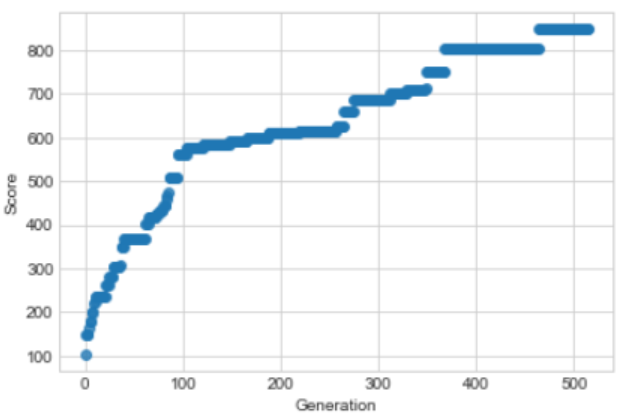
\includegraphics[scale=0.5]{9rows_converge.png}
    \caption{Fitness scores from learner at 9 rows}
    \label{score_9rows}
\end{figure}


\begin{figure}[h]
    \centering
    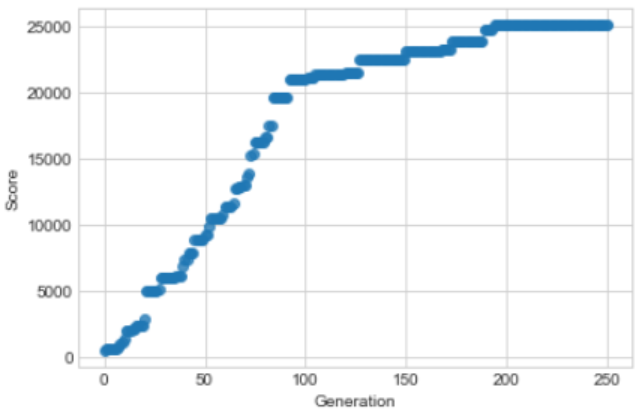
\includegraphics[scale=0.5]{13rows_converge.png}
    \caption{Fitness scores from learner at 13 rows}
    \label{score_13rows}
\end{figure}

Figure \ref{score_histogram} are from the weights shown in Table \ref{feature_weights}.
These weights were derived from the genetic algorithm learner on a board with 13 rows
at generation 132. These were the best set of weights in terms of fitness score from the 13 row learner at the time
the 9 row learner reached convergence at generation 464. 

\begin{table}[h]
    \begin{tabular}{|l|l|}
        \hline
        \textbf{Features}   & \textbf{Weights}     \\
        \hline
        NUM\_ROWS\_REMOVED  & -0.109941154 \\
        \hline
        MAX\_HEIGHT         & -0.115469783  \\
        \hline
        TOTAL\_HEIGHT       & -0.043905252 \\
        \hline
        TOTAL\_DIFF\_HEIGHT & 0.0179129081 \\
        \hline
        LANDING\_HEIGHT     & -0.304447670  \\
        \hline
        NUM\_HOLES          & -0.386174735 \\
        \hline
        COL\_TRANSITION     & -0.125186298 \\
        \hline
        ROW\_TRANSITION     & -0.228061778 \\
        \hline
        COVERED\_GAPS       & -0.769605890  \\
        \hline
        TOTAL\_WELL\_DEPTH  & -0.193777505 \\
        \hline
        HAS\_LOST           & 0.1367227149  \\
        \hline
    \end{tabular}
    \caption{Respective Weights for Features}
    \label{feature_weights}
\end{table}

The result of running 600 games can be seen in Figure \ref{score_histogram},
while some common metrics of the 600 games can be seen on Table \ref{metric_scores}.

\begin{figure}[h]
    \centering
    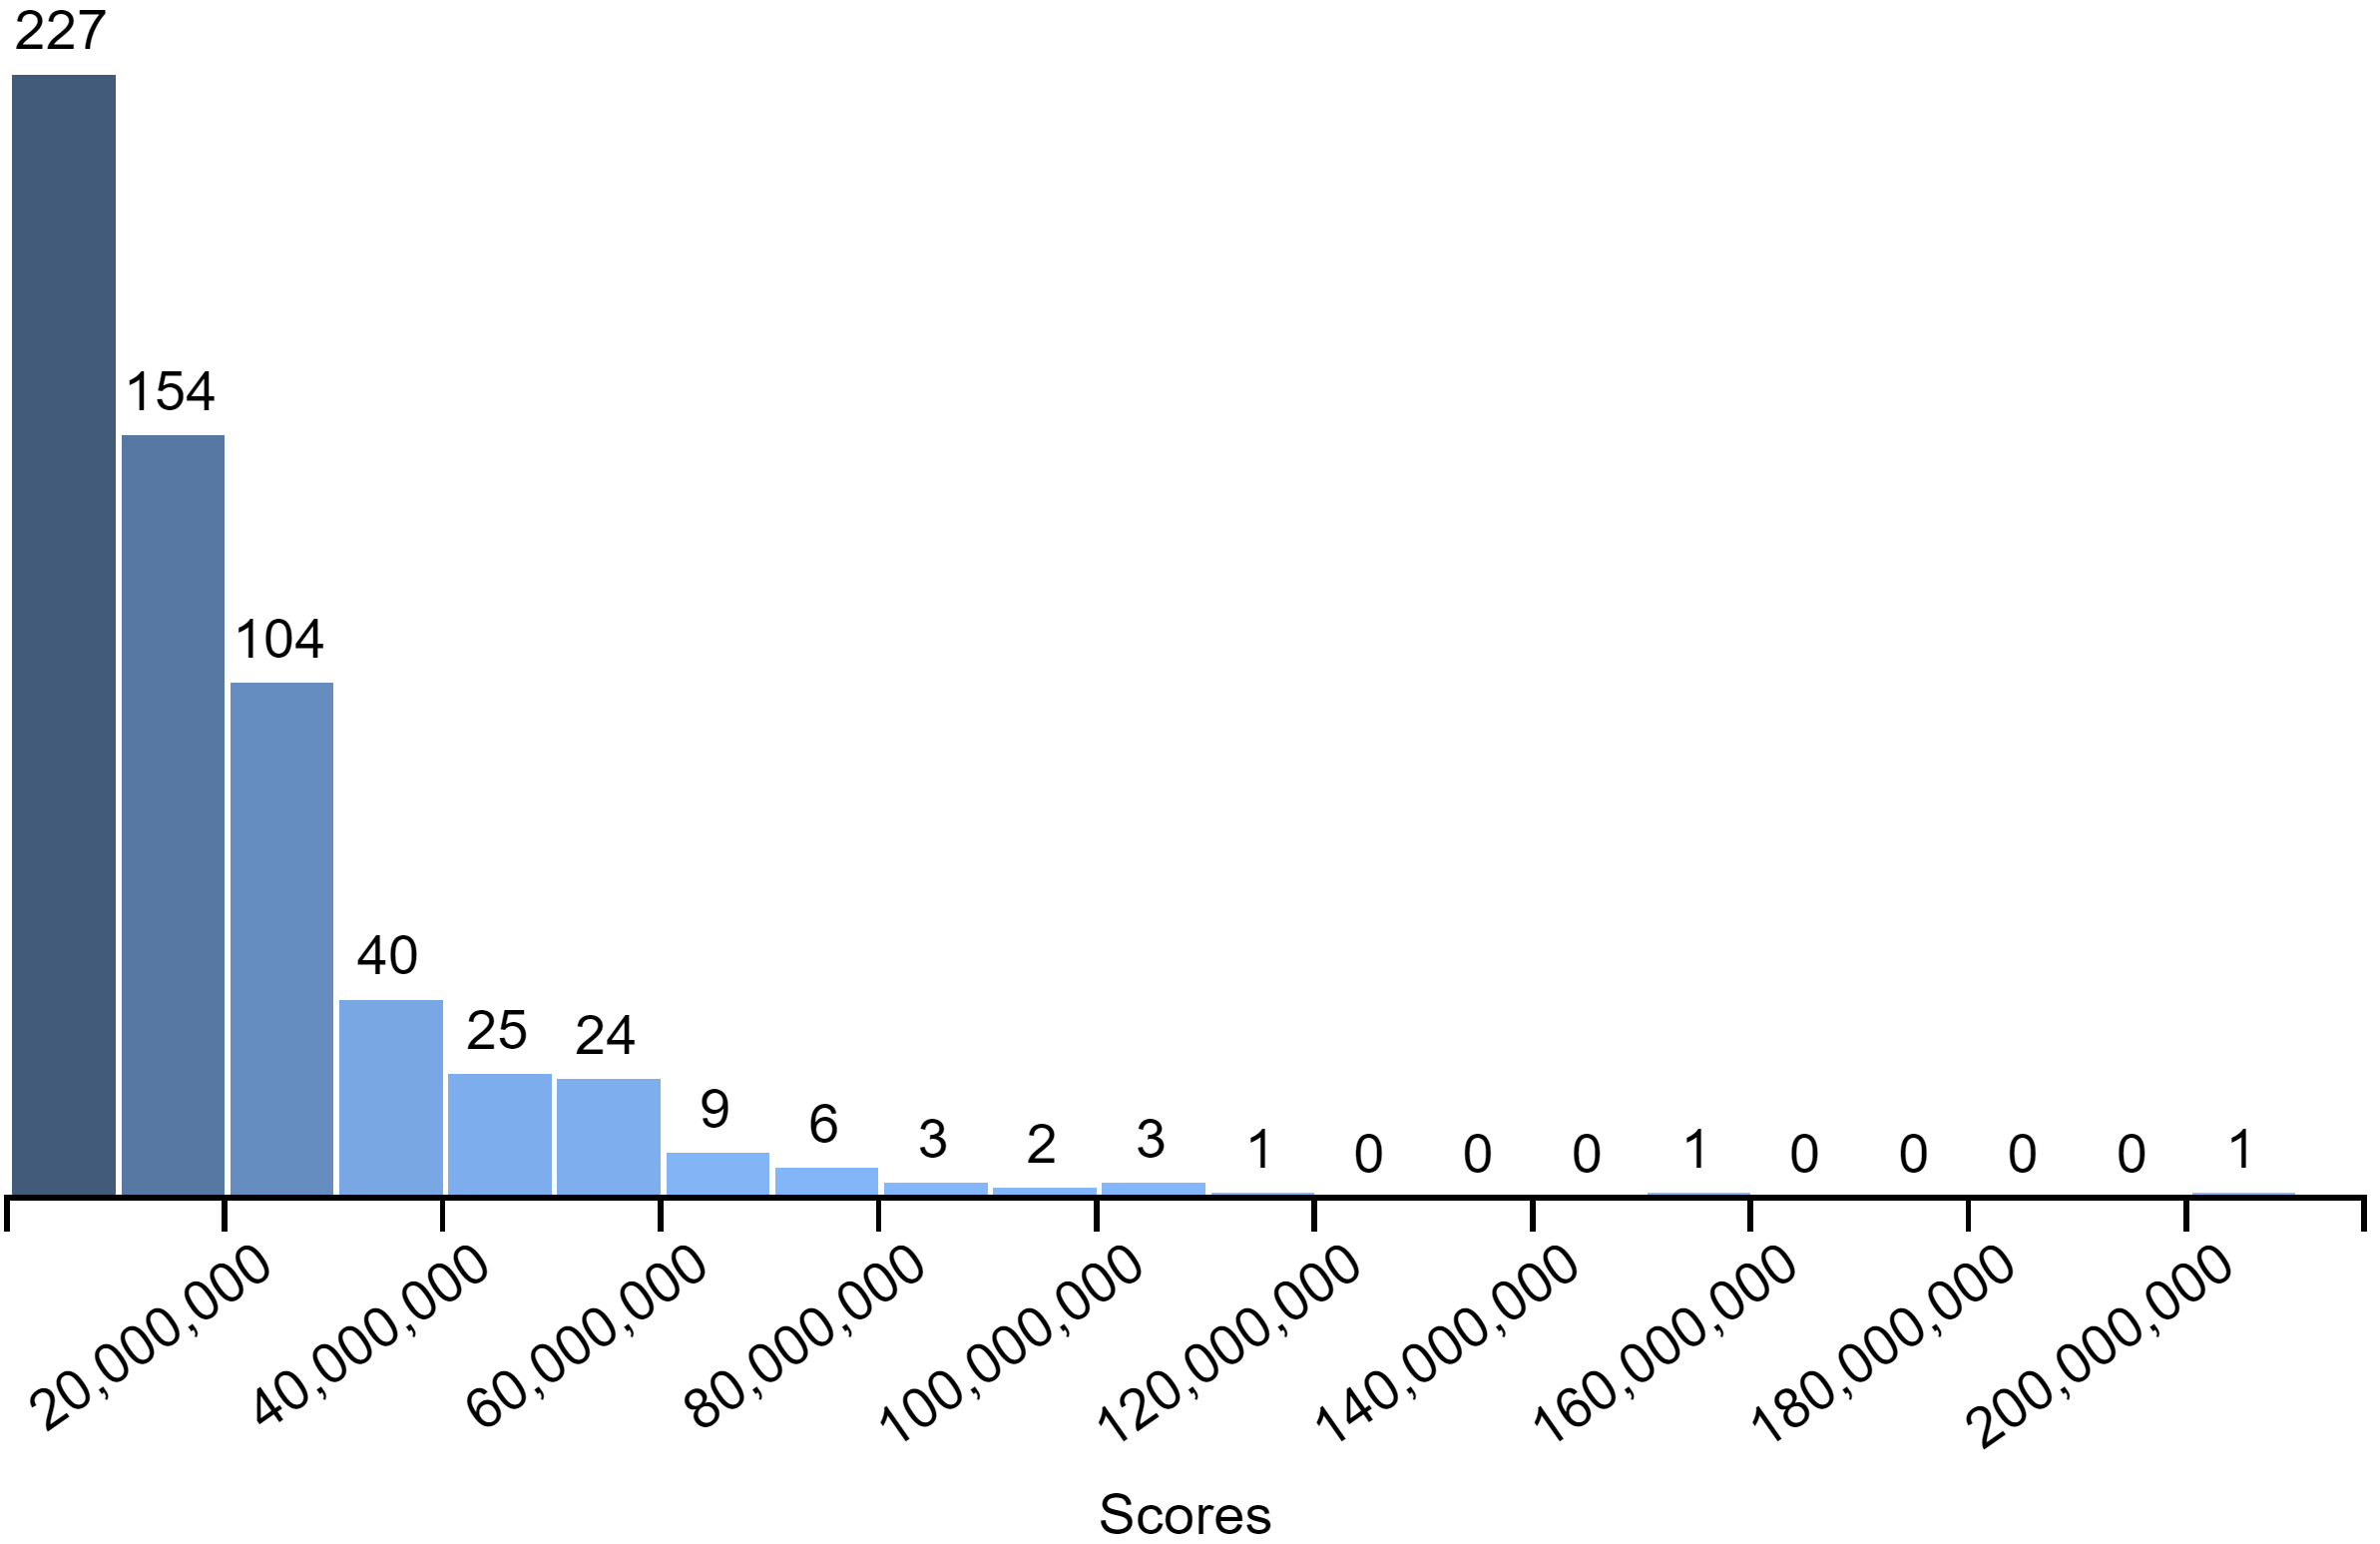
\includegraphics[scale=0.15]{games_600_histogram.png}
    \caption{Results from 600 games}
    \label{score_histogram}
\end{figure}

\begin{table}[h]
    \centering
	\begin{tabular}{|c|c|}
		\hline
		\textbf{Metrics}   & \textbf{Score}     \\
		\hline
		Q1 (25th Percentile)  & 6,307,657.5 \\
		\hline
		Median         & 13,655,622.0  \\
		\hline
		Q3 (75th Percentile)      & 25,716,898.5 \\
		\hline
		Mean & 19,793,958.2 \\
		\hline
		Max     & 216,319,742.0  \\
		\hline
		Min          & 5125.0 \\
		\hline
	\end{tabular}
	\caption{Common Metrics for the Scores}
	\label{metric_scores}
\end{table}

As we can see from the result, most of the games played lie below 30 million lines
cleared. However we do see a few outliers that broke 50 million lines cleared, including
our best run at 216,319,742 lines cleared.

\section{Discussion and Findings}
\label{discussion_n_findings}
Our group initially decided to use Least Square Policy Iteration (LSPI) by Lagoudakis \cite{lagoudakis},
as our learning algorithm because we found that earlier CS3243 groups such as
Tan et al \cite{shawntan} and Nguyen et al \cite{nhannguyen} had been able to get
satisfactory results from it. However, the results that we have produced from our
implementation of LSPI was not satisfactory, giving an average of at most 8,000 rows
cleared.

We speculated that there may have been an error in our implementation, but despite
peer review, we were not able to find the issue. In an attempt to try to improve the
learnt weights, we tried implementing other features to better represent the state
of the board. This was when our team realised the importance of the choice of features.

We initially implemented our original set of features without HAS\_LOST. Most of which
was taken from previous other works of tetris playing agents, such as the Tetris
applications by Colin Fahey and Pierre Dellacherie \cite{colin_fahey}, because of
how well those features had worked.

However, those features do not take in account of whether the next move will result
in a loss, therefore an important characteristic of the board has not been captured.
Implementing HAS\_LOST will discourages our agent from making losing moves if
there are other available non-losing moves.

After implementing this feature, the number of rows cleared on the average increased
from 8,000 to 80,000. Nonetheless, the results were still unsatisfactory and the team
decided to change the implementation of the learner to use our own version of genetic
algorithm instead.

\begin{table}[h]
	\centering
	\begin{tabular}{|l|l|}
		\hline
		\textbf{Metrics}                 & \textbf{Mean Score} \\
		\hline
		13 Rows Learner (Generation 132) & 19,793,958.2        \\
		\hline
		9 Rows Learner (Generation 464)  & 12,872,842.8        \\
		\hline
	\end{tabular}
	\caption{
		Comparison of the final top weights of each learner after 9 rows learner
		reached convergence
	}
	\label{learner_comparison}
\end{table}

With regards to the 2 instances of learners running on 9 and 13 rows respectively.
We found that the learner on the 9x10 board has converged much faster than the
learner on the 13x10 board. However, testing on a full sized 20x10 board with 600 games,
the player trained on the larger board gave a higher mean score than the player
trained on a smaller board, as can be seen in Table \ref{learner_comparison}.

The apparent tradeoff for this speed up in convergence, is that the set of weights
obtained are not ideal for a full sized board, though the player still plays well.
We think that learning on a smaller game board may be specialising the player for playing on
a smaller game board size but does not enable them to generalise to larger game board sizes.

This illustrates the tradeoff between tweaking the size of the board (to
reduce the time taken for convergence), as well as the quality of the weights
learnt at the end, which would be another interesting area to look into if we had
more time.

\section{Further Considerations}

In addition to the discussion on Section \ref{parallelisation_n_speedup},
another possible way that we could look into speeding up the fitness evaluation
of each chromosome is by reducing the length of each game. If the player has reached
the maximum number of moves made or has lost, report the score. However, this may
lead to a set of weights that are specialised in playing only up to the maximum
number of moves and not anymore. The combination of states that the player sees may
also be biased to the states that are closer to the start of a game, thus not
giving an evaluation that can be generalised to a standard game. Hence how we
tweak the maximum number of moves made would be crucial in balancing the
time taken versus quality of weights learnt.

Lastly, we can further parallelise the running of the genetic algorithm by distributing
the fitness evaluation of each chromosome to separate machines in different
clusters. This will decrease the computational time needed for each generation as the
fitness evaluation for all chromosomes would now be running in parallel in different
machines.

\section{Conclusion}
In this paper, we used Genetic Algorithm to arrive at a strategy for a utility based
agent that could play Tetris well. This strategy derived could then be used as good
starting point in another algorithm such as LSPI, in order to learn the optimal weights,
as our Tetris problem could be tailed to fit a control problem as stated by Lagoudakis \cite{lagoudakis}.

We also looked at different methods of making the algorithm learn a good strategy faster,
such as reducing the size of the board, and its various tradeoffs.
% Our aim in this paper was to show we can use Genetic Algorithm to apply to strategies
% in terms of weights to our feature-based utility function to evaluate the best moves.
% We have showed that the algorithm could settle at a good set of weights, despite
% not having a guarantee that each consecutive generation would improve. The set of weights
% that we have derived based on these features could then be used in as a starting point
% in another algorithm in order to learn the optimal weights, such as LSPI, of which our
% Tetris problem could be be tailored to fit a control problem as stated by Lagoudakis \cite{lagoudakis}.

% We have shown that by reducing the size of the game board, we could still arrive at
% a set of weights that were decent. We discussed the tradeoff of reducing
% the size of the board, and the final weight's ability to generalise to larger
% board sizes. We also examined other ways to reduce the length of games and its
% possible implications on how generalisable the weights learnt at the end will be.

As a final concluding point, we think that in order to design a utility based agent
that could play Tetris well, we should not rely on only optimising the weights
for a set of features, we should also be looking into selecting good features as well.
As discussed in Section \ref{discussion_n_findings}, having a set of features that
could better represent the state of the game, results in an agent that plays better.
Perhaps another interesting area to research would be looking into creating algorithms
that could optimise and learn new features of the board state, and thus the utility
function, instead of just optimising its weights.

\begin{thebibliography}{9}
    \bibitem{shawntan}
    Shawn Tan et al, \textit{Learning about reinforcement learning, with Tetris}, 2014\\https://blog.wtf.sg/2014/01/12/learning-about-reinforcement-learning-with-tetris/

    \bibitem{nhannguyen}
    Nhan Nguyen et al, \textit{Learning to Play Tetris with Big Data}, 2016\\https://github.com/ngthnhan/Tetris/blob/final/report.pdf

    \bibitem{colin_fahey}
    Colin P. Fahey, \textit{Tetris AI}, 2003\\https://www.colinfahey.com/tetris/tetris.html
    
    \bibitem{lagoudakis}
    Michail G. Lagoudakis, Ronald Parr.
    \textit{Journal of Machine Learning Research 4 (Dec), 1107-1149}, 2003
\end{thebibliography}

\end{document}
